\documentclass[usenames,dvipsnames]{beamer}
\usetheme{Boadilla}
\usepackage{hyperref}
\usepackage{graphicx}
\usepackage{multimedia}
\usepackage{fancyvrb}
\usepackage{soul}
\usepackage{multicol}
\usepackage{optparams}
\usepackage{adjustbox}
\usepackage{tikz}
\usetikzlibrary{shapes,positioning}
\newcommand{\foo}{\hspace{-2.3pt}$\bullet$ \hspace{5pt}}
\usepackage{subfig}
\usepackage[
    backend=biber,
    natbib=true,
    style=numeric,
    sorting=none,
    style=verbose-ibid,
    maxcitenames=1, %remove this outside of toy presentations
]{biblatex}
\addbibresource{citations.bib}
\usepackage{pgfpages}
\usepackage{xcolor}
\definecolor{ao(english)}{rgb}{0.0, 0.5, 0.0}
\definecolor{burgundy}{rgb}{0.5, 0.0, 0.13}
%\setbeameroption{show notes}
%\setbeameroption{show notes on second screen=right}
\setbeameroption{hide notes}
\newcommand\ThesisTitle{Music Source Separation with the sliCQ Transform}


\title{Improving Open-Unmix for Music Source Separation}
\subtitle{Brainstorming session}
\author{Sevag Hanssian}
\institute{DDMAL, McGill}
\setbeamertemplate{navigation symbols}{}

\AtEveryBibitem{%
  \clearfield{pages}%
  \clearfield{volume}%
  \clearfield{number}%
  \clearlist{journal}%
  \clearfield{booktitle}%
}

\renewbibmacro{in:}{}

\AtEveryCitekey{%
  \clearfield{pages}%
  \clearfield{volume}%
  \clearfield{number}%
  \clearfield{doi}%
  \clearfield{journal}%
  \clearlist{journal}%
  \clearfield{booktitle}%
  \clearfield{isbn}%
  \clearfield{title}%
  \clearfield{url}%
\ifentrytype{article}{
    \clearfield{journal}%
}{}
\ifentrytype{inproceedings}{
    \clearfield{booktitle}%
}{}
}

\begin{document}

\begin{frame}
\maketitle
\end{frame}


\begin{frame}
	\adjustbox{valign=c}{{\usebeamerfont{frametitle}\usebeamercolor[fg]{frametitle}Timeline}}\hfill
	\adjustbox{valign=c}{
	\newcounter{year}
	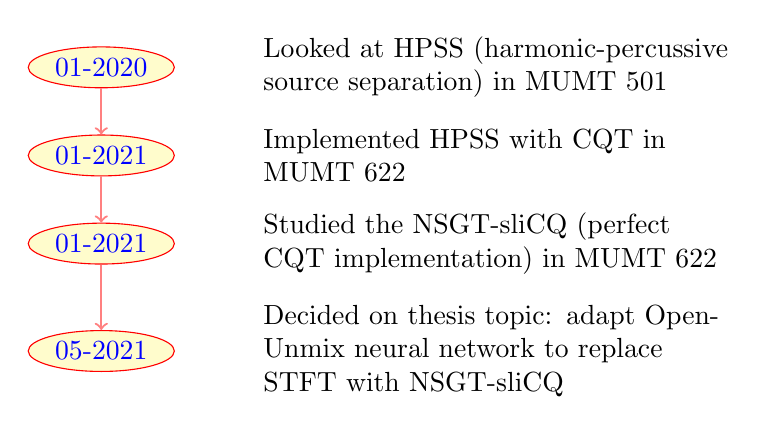
\begin{tikzpicture}[yscale=0.5,%
		   year/.style={draw=red,text=blue,fill=yellow!20,shape=ellipse,inner sep=2pt},
		   description/.style={rectangle,align=left,text width=60mm,anchor=west},
		   timeline/.style={->,thick,red!50}]

	    \foreach \year/\desc [count=\y] in {%
	       01-2020/Looked at HPSS (harmonic-percussive source separation) in MUMT 501,%
	       01-2021/Implemented HPSS with CQT in MUMT 622,%
		01-2021/Studied the NSGT-sliCQ (perfect CQT implementation) in MUMT 622,%
	       05-2021/Decided on thesis topic: adapt Open-Unmix neural network to replace STFT with NSGT-sliCQ%
	       } { \ifnum\y=1 \node[description](\y){\desc};
		   \else\node[description,below=1ex of \z](\y){\desc};
		   \fi
		   \node[year](y-\y) [left=of \y] {\year};
		   \ifnum\y>1\draw[timeline] (y-\z)-- (y-\y);\fi
		   \global\let\z=\y% for drawing from last node
	       }

	\end{tikzpicture}
	}
\end{frame}

\begin{frame}
	\frametitle{Competition}
	By pure luck, there is a May-August 2021 competition by the creators of Open-Unmix: \href{https://www.aicrowd.com/challenges/music-demixing-challenge-ismir-2021}{https://www.aicrowd.com/challenges/music-demixing-challenge-ismir-2021}\\
	\includegraphics[height=2.5cm]{./challenge.png}\\
	Deadlines:
	\begin{enumerate}
		\item
			\st{Round 1: May 3rd - June 13th, 12 PM UTC} - hidden dataset A, already finished
		\item
			Round 2: June 14th - July 31st, 12 PM UTC - hidden dataset B
		\item
			Team Freeze deadline: 23rd July, 12 PM UTC
	\end{enumerate}
	All submissions get evaluated on a full hidden dataset in August (meaning I have until July 31 to submit a winner)
\end{frame}

\begin{frame}
	\frametitle{Competition pt2}
	I made 1 submission to Round 1: tiny tweaks (LSTM $\rightarrow$ GRU, swap batchnorm and activations, etc.), added my Periphery stems (4 albums) dataset to MUSDB18-HQ to try to train with extra metal data\\
	\includegraphics[height=4cm]{./top5.png}
	\includegraphics[height=2.17cm]{./currentplace.png}
\end{frame}

\begin{frame}[fragile]
	\frametitle{Music Source Separation}
	\begin{enumerate}
		\item
			When producing music, instruments are recorded separately (aka stems), and combined (linear mixture) to make mixed song -- commonly 4 sources, bass, drums, vocals, other, deriving from MUSDB18-HQ dataset \footcite{musdb18hq}, e.g.:
			\begin{verbatim}
			# ls MUSDB18-HQ/train/Night\ Panther\ -\ Fire/
			vocals.wav mixture.wav drums.wav other.wav bass.wav
			\end{verbatim}
		\item
			On the flip side, given a mixed song, we want to decompose it back into its stems (without having access to the stems)
	\end{enumerate}
	\begin{figure}[ht]
		\centering
		\subfloat{\includegraphics[height=2.5cm]{./mixing.png}}
		\hspace{0.1em}
		\subfloat{\includegraphics[height=2.5cm]{./demixing.png}}
		\caption{Mixing and ``demixing'' or source separation}
	\end{figure}
\end{frame}

\begin{frame}[fragile]
	\frametitle{Neural networks for Music Source Separation}
	\begin{enumerate}
		\item
			\textbf{Ground truth:} source stems that are combined to make mixed song -- commonly 4 sources, bass, drums, vocals, other. Also very commonly 1 network per source
		\item
			\textbf{Network inputs:} mixed waveform and 1 source -- direct waveform, or a TFR (time-frequency representation)  e.g. STFT
		\item
			\textbf{Estimate source:} given the mixed input, learn how to extract a source. Common approach: learnable magnitude-STFT mask, e.g. same shape as spectrogram but $\in [0.0, 1.0]$, to multiply mixed spectrogram with
		\item
			\textbf{Back to waveform:} after estimating the source, convert it back to waveform -- can use masking or mix-phase inversion. Mixture supplies the STFT phase, estimates only use magnitude
	\end{enumerate}
\end{frame}

\begin{frame}
	\frametitle{Visualizations}
	\begin{figure}[ht]
		\includegraphics[height=2.5cm]{./mask_simple.png}
		\caption{Example of a binary mask applied to an STFT}
	\end{figure}
	\begin{figure}[ht]
		\includegraphics[height=2.5cm]{./whynophase.png}
		\caption{Why we don't try to learn phase in neural networks}
	\end{figure}
\end{frame}

\begin{frame}
	\frametitle{Open-Unmix}
	Very open source, near-SOTA music source separation. Intended to be a ``platform'' for future MSS research.
	\begin{figure}[ht]
		\includegraphics[height=3cm]{./umx1.png}
		\caption{Open-Unmix diagram}
	\end{figure}
	UMX estimates source magnitude STFT with a nonnegative mask (ReLU)\\
	4 networks, 1 per source (bass, drums, vocals, other)
\end{frame}

\begin{frame}
	\frametitle{Getting the stem waveform}
	Recall: output of unmix is the estimated \textbf{magnitude STFT} of the vocal stem\\\ \\

	Open-unmix uses phase of mixture:
	\begin{enumerate}
		\item
			\textbf{x, inference:} x = mix waveform
		\item
			\textbf{Estimate Ymag, vocals:}\\
			\qquad $X_{\text{mag}} = abs(\text{STFT}(x))$, $\hat{Y}_{\text{mag}} = \text{network}(X_{\text{mag}})$
		\item
			\textbf{Mix phase inversion:}\\
			\qquad $X_{\text{phase}} = atan2(\text{STFT}(x))$\\
			\qquad $\hat{Y}_{\text{complex}} = \hat{Y}_{\text{mag}} + j X_{\text{phase}} \rightarrow \hat{y} = \text{iSTFT}(\hat{Y}_{\text{complex}})$
		\item
			Evaluation: BSS (SDR, SAR, SIR, ISR) on $\hat{y}, y_{\text{groundtruth}}$
	\end{enumerate}
\end{frame}

\begin{frame}
	\frametitle{Oracle, or ideal, performance}
	Mix phase oracle (hasn't been evaluated before). Given ground truths, \textbf{how good can source separation be?} Assuming a perfect estimate from the neural network\\

	Using ground-truth instead of network predictions:
	\begin{enumerate}
		\item
			\textbf{x, y ground truth:} x = mix waveform, y = vocals
		\item
			\textbf{Ideal mix phase inversion:}\\
			\qquad $X_{\text{phase}} = atan2(\text{STFT}(x))$\\
			\qquad $Y_{\text{mag}} = abs(\text{STFT}(y))$\\
			\qquad $Y_{\text{ideal complex}} = Y_{\text{mag}} + j X_{\text{phase}} \rightarrow y_{\text{ideal}} = \text{iSTFT}(Y_{\text{ideal complex}})$
		\item
			Evaluation: BSS (SDR, SAR, SIR, ISR) on $y_{\text{ideal}}, y_{\text{groundtruth}}$
	\end{enumerate}
\end{frame}

\begin{frame}
	\frametitle{STFT vs. NSGT oracle performance}
	Using SDR only (the most important score):\\
	STFT, UMX default (window = 4096): vocals 8.62, drums 7.07, bass 6.68, other 6.87\\

	NSGT (with maximum slice length capped at 8192 frames):\\

	Bass NSGT = Bark, 105 bins, 25.4-22050 Hz, slice = 7180 = 8.47\\
	Drums NSGT = Mel, 104 bins, 49.3-22050 Hz, slice = 7108 = 10.5\\
	Other NSGT = Bark, 64 bins, 90.0-22050 Hz, slice = 4416 = 13.94\\
	Vocals NSGT = Mel, 116 bins, 37.7-22050 Hz, slice = 8024 = 9.83\\\ \\

	\textbf{Hypothesis}:
	\begin{enumerate}
		\item
			If one can prepare a neural network that can estimate the magnitude-sliCQ-NSGT
		\item
			Then using the above configurations can get significant SDR gains since they perform considerably better in the mix-phase oracle
		\item
			UMX-STFT: estimate abs(STFT-4096) $\rightarrow$ \\
			\qquad UMX-NSGT: estimate abs(NSGT-Bark-105-25.4Hz-7180)
	\end{enumerate}
\end{frame}

\begin{frame}
	\frametitle{sliCQ in UMX, dimensionality visuals}
	\includegraphics[height=6.5cm]{./umxslicqdimred.png}
\end{frame}

\begin{frame}
	\frametitle{NSGT-sliCQ inside Open-Unmix}
	NSGT-sliCQ choices:
	\begin{itemize}
		\item
			Reduce to 2d (overlap-add or flatten) -- same dimensionality as an STFT
		\item
			Treat as 3-dimensional sequence of 2d time-frequency frames!\\
			2-d spectrogram = image (RGB x width x height $\rightarrow$ mono/stereo x time x frequency)\\
			3-d sliCQ = video (temporal frame x mono/stereo x (2d time x frequency)\\
			$\text{Slice} \times (\text{Frequency} \times \text{Time-in-slice})$
	\end{itemize}
	Input size:
	\begin{enumerate}
		\item
			input stft, 6s audio = abs(STFT(4096)) = $258 \times 2049 \approx 500,000$
		\item
			input slicq, 6s audio = abs(sliCQ(mel,116,37.7)) = $67 \times 117 \times 244 \approx 1,912,716$
		\item
			UMX has ~1 million parameters for 500,000-sized input. Scale accordingly? Do I necessarily need a model that has 4 million parameters, or similar?
		\item
			Leaning towards CNN for large, structured inputs
	\end{enumerate}
\end{frame}

\begin{frame}
	\frametitle{STFT in UMX, visual}
	\includegraphics[height=3cm]{./umxstftlstm.png}
\end{frame}


\begin{frame}
	\frametitle{sliCQ in UMX LSTM, option 1}
	\includegraphics[height=2.7cm]{./umxslicqlstm1.png}\\
	\textbf{nb:} overlap version is non-invertible
\end{frame}

\begin{frame}
	\frametitle{sliCQ in UMX LSTM, option 2}
	\includegraphics[height=2.7cm]{./umxslicqlstm2.png}
\end{frame}

\begin{frame}[fragile]
	\frametitle{Debugging ideas}
	The ``golden test'': overfit to 2 training examples (2x 6s segments) + 1 validation example (1x 12s segment)
	\begin{verbatim}
        /home/sevagh/musdbdebug/
        └── train
            ├── Actions - One Minute Smile
            ├── Night Panther - Fire
            └── Steven Clark - Bounty
	\end{verbatim}
	Gradient debugging with Tensorboard
\end{frame}

\begin{frame}
	\frametitle{Resources}
	umx-junkyard: all my wild experiments (conv2d,3d,4d, lstm, gru, dilations, maxpools, etc.)\\
	\includegraphics[height=6cm]{./junkyard.png}\\
	easy to copy-paste blocks of code from various configurations
\end{frame}

\begin{frame}
	\frametitle{Golden test -- overfit 2 training + 1 validation}
	Tensorboard plots:
	\begin{enumerate}
		\item
			Loss: MSE
		\item
			SDR: SI-SDR (true source separation performance)\\
			(tried this as loss function but it's very computationally expensive w.r.t gradients)
		\item
			Audio clips of source separation
		\item
			Plots of 3D magnitude sliCQ coefficients (input x y and y est) -- using TSNE for 3d
		\item
			Also 2d spectrogram from sliCQ
	\end{enumerate}
\end{frame}

\begin{frame}
	\frametitle{Open-Unmix with 2d sliCQ + LSTM}
	UMX-sliCQ 2d:
	\begin{enumerate}
		\item
			\textbf{x, y training example:} x = mix waveform, y = vocal stem (6 second sequence)
		\item
			\textbf{Network:} magnitude NSGT = $abs(NSGT(x))$ = $\text{Slices} \times \text{Frequency} \times \text{Time-in-slice}$\\E.g. for NSGT-mel-115-37.7hz, on 6 seconds of audio = $67 \text{ slices} \times 117 \text{ frequencies} \times 244 \text{ time-in-slice bins} $
		\item
			\textbf{Flatten:} $67 \text{ slices} \times 117 \text{ frequencies} \times 244 \text{ time-in-slice bins} \rightarrow 16384 \text{ time} \times 117 \text { frequencies}$\\
			\textbf{\textcolor{red}{LSTMs can deal with overlapping sequences, right?}}
		\item
			\textbf{Recurrence}: BLSTM, hidden = 117, 3 layers, dropout + skip-conn\\
			16384 frames of 117 frequencies pass through the LSTM\\
			\textbf{contrast with} 258 frames of 512 compressed frequencies of STFT
			\textbf{\textcolor{red}{huge sequence length is not good -- slow training, bad gradients, never worked for me}}
	\end{enumerate}
\end{frame}

\begin{frame}
	\frametitle{Open-Unmix with 3d sliCQ + LSTM}
	UMX-sliCQ 3d:
	\begin{enumerate}
		\item
			\textbf{x, y training example:} x = mix waveform, y = vocal stem (6 second sequence)
		\item
			\textbf{Network:} magnitude NSGT = $abs(NSGT(x))$ = $\text{Slices} \times \text{Frequency} \times \text{Time-in-slice}$\\E.g. for NSGT-mel-115-37.7hz, on 6 seconds of audio = $67 \text{ slices} \times 117 \text{ frequencies} \times 244 \text{ time-in-slice bins} $
		\item
			\textbf{Flatten differently:} $67 \text{ slices} \times 117 \text{ frequencies} \times 244 \text{ time-in-slice bins} \rightarrow 67 \text{ slices} \times (117 \text { frequencies} \times 244 \text { time-in-slice} = 28548)$\\
			\textbf{LSTM is now taking the temporally evolving sequence of ``1D'' flattened sliCQ tf frames)}
		\item
			\textbf{Recurrence}: BLSTM, hidden = 28548, 3 layers, dropout + skip-conn\\
			67 frames of 27378 sliCQ coefficients pass through the LSTM\\
			\textbf{contrast with} 258 frames of 512 compressed frequencies of STFT
			\textbf{\textcolor{red}{reducing the 1D dimensionality to not have a hidden size of 28548 -- linear encoder?}}
	\end{enumerate}
\end{frame}

\begin{frame}
	\frametitle{Open-Unmix with 3d sliCQ + Conv-LSTM}
	UMX-sliCQ 3d:
	\begin{enumerate}
		\item
			\textbf{x, y training example:} x = mix waveform, y = vocal stem
		\item
			\textbf{Network:} magnitude NSGT = $abs(NSGT(x))$ = $\text{Slices} \times \text{Frequency} \times \text{Time-in-slice}$\\E.g. for NSGT-mel-115-37.7hz, on 6 seconds of audio = $67 \text{ slices} \times 117 \text{ frequencies} \times 244 \text{ time-in-slice bins} $
		\item
			\textbf{Conv3d encoder:} Use $1 \times T \times F$ kernels to not touch the slice/temporal dimension:\\
			$67 \text{ slices} \times 117 \text{ frequencies} \times 244 \text{ time-in-slice bins} \rightarrow$ strided convolution layers $\rightarrow 67 \text{ slices} \times (6 \text { fconv} \times 10 \text { tconv} = 60)$\\
			\textbf{LSTM is now taking the temporally evolving sequence of ``1D'' flattened convencoder(sliCQ)}
		\item
			\textbf{Recurrence}: BLSTM, hidden = 60, 3 layers, dropout + skip-conn\\
			67 frames of 60 conv3d(sliCQ) coefficients pass through the LSTM
		\item
			\textbf{ConvTranspose3d decoder:} grow $60 = 6 \times 10$ back to $117 \times 244$

			\textbf{``feels right'' but doesn't generalize - \textcolor{red}{convolution parameter selection - kernels, layers, hidden channels}}
	\end{enumerate}
\end{frame}

\begin{frame}
	\frametitle{Open-Unmix with 3d sliCQ + Convolutions, no LSTM}
	UMX-sliCQ 3d:
	\begin{enumerate}
		\item
			\textbf{x, y training example:} x = mix waveform, y = vocal stem (6 second sequence)
		\item
			\textbf{Network:} magnitude NSGT = $abs(NSGT(x))$ = $\text{Slices} \times \text{Frequency} \times \text{Time-in-slice}$\\E.g. for NSGT-mel-115-37.7hz, on 6 seconds of audio = $67 \text{ slices} \times 117 \text{ frequencies} \times 244 \text{ time-in-slice bins} $
		\item
			\textbf{Conv3d encoder:} Use $S \times T \times F$ kernels to also find patterns across the slice dimension
			$67 \text{ slices} \times 117 \text{ frequencies} \times 244 \text{ time-in-slice bins} \rightarrow$ strided convolution layers $\rightarrow 4 \text{ slices} \times (6 \text { fconv} \times 10 \text { tconv} = 60)$\\
		\item
			\textbf{ConvTranspose3d decoder:} grow $4 \times 6 \times 10$ back to $67 \times 117 \times 244$
	\end{enumerate}
	\textbf{\textcolor{red}{based more on Convolutional autoencoder/decoder theory, not an adaptation of UMX anymore}}\\
	\textbf{\textcolor{red}{no luck}}\\
\end{frame}

\end{document}
